\documentclass[xcolor=svgnames]{beamer}
\usetheme{Torino}

\usepackage{epsfig} %for figures
\usepackage{xcolor} %for color
\usepackage[utf8]{inputenc}

% latex definitions:
\def\d{{\rm d}}
\def\half{{\textstyle{1\over2}}}



\title[SymPy\hspace{4em}\insertframenumber/
\inserttotalframenumber]{~\\ SymPy Tutorial \\~}


\author[O. Čertík, M. Paprocki, A. Meurer]
{Ondřej Čertík, Mateusz Paprocki, Aaron Meurer}

\pgfdeclareimage[height=1.5cm]{mylogo}{sympy-250px}
\institute{\pgfuseimage{mylogo}}

\date{June 24, 2013}

\begin{document}

\begin{frame}
  \maketitle
\end{frame}

\begin{frame}{Outline}
  \begin{block}{SymPy Introduction}
    \begin{itemize}
    \item Goal
    \item History
    \item Current status
    \item Features
    \end{itemize}
  \end{block}

  \begin{block}{Tutorial}
    \begin{itemize}
    \item Basic SymPy commands
    \item Solving real life problems
    \end{itemize}
  \end{block}
\end{frame}

\begin{frame}{SymPy Goal}
  \begin{block}{Goal}
    Provide symbolic manipulation library in Python.
  \end{block}
  \pause
  \begin{block}

    ``SymPy is an open source Python library for symbolic mathematics. It aims to
    become a full-featured computer algebra system (CAS) while keeping the code as
    simple as possible in order to be comprehensible and easily extensible. SymPy
    is written entirely in Python and does not require any external libraries.''

  \end{block}
\end{frame}

\begin{frame}{History}
  \begin{block}{History}
    \begin{itemize}
    \item Ondřej Čertík started the project in 2006.
    \item Development took off in 2007 when SymPy first participated in Google
      Summer of Code. We have participated in every Google Summer of Code since.
    \item In 2011, Aaron Meurer (who also joined from Google Summer of Code) took
      over as lead developer.
    \end{itemize}
  \end{block}
\end{frame}

\begin{frame}
  \begin{block}{Current Status}
    \begin{itemize}
    \item Over 250 contributors.
    \item Current code base has over 400,000 lines of code and documentation.
    \end{itemize}
  \end{block}
\end{frame}

\begin{frame}{Git Commits Plots}
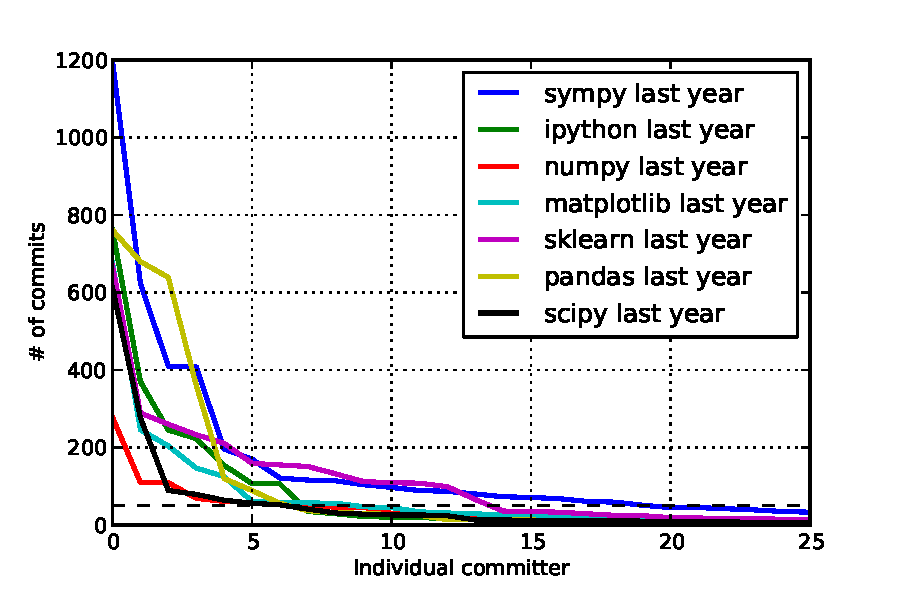
\includegraphics[width=4in]{commits1.pdf}
\end{frame}

\begin{frame}{Git Commits Plots (normalized)}
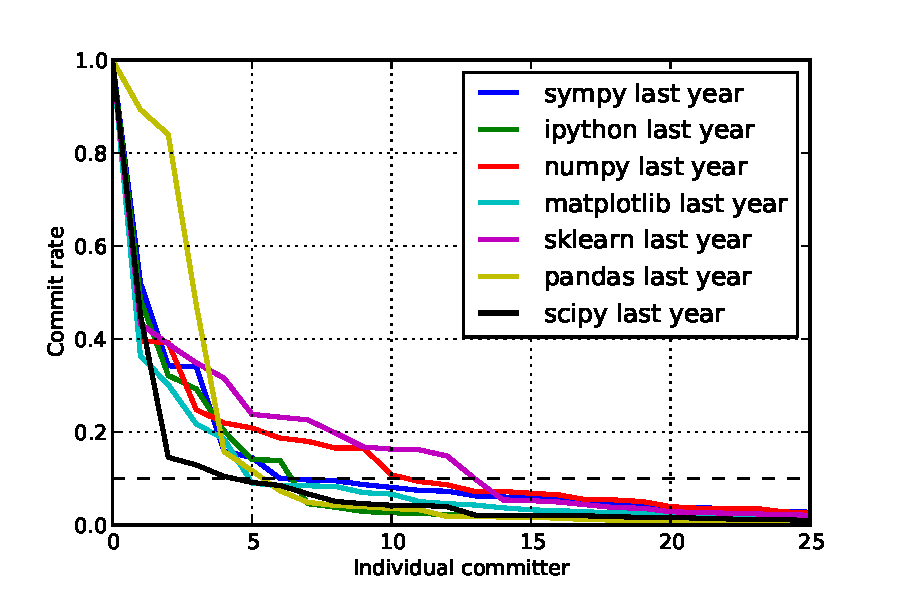
\includegraphics[width=4in]{commits2.pdf}
\end{frame}

\begin{frame}{Features}
  \begin{block}{Core capabilities}
    \begin{itemize}
    \item Basic arithmetic: Support for operators such as +, -, *, /, ** (power)
    \item Simplification
    \item Expansion
    \item Functions: trigonometric, hyperbolic, exponential, roots, logarithms,
      absolute value, spherical harmonics, factorials and gamma functions, zeta
      functions, polynomials, special functions, \ldots
    \item Substitution
    \item Numbers: arbitrary precision integers, rationals, and floats
    \item Noncommutative symbols
    \item Pattern matching
    \end{itemize}
  \end{block}
\end{frame}

\begin{frame}{Features}
  \begin{block}{Polynomials}
    \begin{itemize}
    \item Basic arithmetic: division, gcd, \ldots
    \item Factorization
    \item Square-free decomposition
    \item Gröbner bases
    \item Partial fraction decomposition
    \item Resultants
    \end{itemize}
  \end{block}
\end{frame}

\begin{frame}{Features}
  \begin{block}{Calculus}
    \begin{itemize}
    \item Limits: $$\lim_{x\to 0}{x\log(x)} \rightarrow 0$$
    \item Differentiation
    \item Integration: It uses extended Risch-Norman heuristic
    \item Taylor (Laurent) series
    \end{itemize}
  \end{block}
\end{frame}

\begin{frame}{Features}
  \begin{block}{Solving equations}
    \begin{itemize}
    \item Polynomial equations
    \item Algebraic equations
    \item Differential equations
    \item Difference equations
    \item Systems of equations
    \end{itemize}
  \end{block}
\end{frame}

\begin{frame}{Features}
  \begin{block}{Combinatorics}
    \begin{itemize}
    \item Permutations
    \item Combinations
    \item Partitions
    \item Subsets
    \item Permutation Groups: Polyhedral, Rubik, Symmetric, \ldots
    \item Prufer and Gray Codes
    \end{itemize}
  \end{block}
\end{frame}

\begin{frame}{Features}
  \begin{block}{Discrete math}
    \begin{itemize}
    \item Binomial coefficients
    \item Summations
    \item Products
    \item Number theory: generating prime numbers, primality testing, integer
      factorization, \ldots
    \item Logic expressions
    \end{itemize}
  \end{block}
\end{frame}

\begin{frame}{Features}
  \begin{block}{Matrices}
    \begin{itemize}
    \item Basic arithmetic
    \item Eigenvalues/eigenvectors
    \item Determinants
    \item Inversion
    \item Solving
    \item Abstract expressions
    \end{itemize}
  \end{block}
\end{frame}

\begin{frame}{Features}
  \begin{block}{Geometric Algebra}
  \end{block}

  \begin{block}{Geometry}
    \begin{itemize}
    \item points, lines, rays, segments, ellipses, circles, polygons, \ldots
    \item Intersection
    \item Tangency
    \item Similarity
    \end{itemize}
  \end{block}
\end{frame}

\begin{frame}{Features}
  \begin{block}{Plotting}
    \begin{itemize}
    \item Coordinate modes
    \item Plotting Geometric Entities
    \item 2D and 3D
    \item Interactive interface
    \item Colors
    \end{itemize}
  \end{block}
\end{frame}

\begin{frame}{Features}
  \begin{block}{Physics}
    \begin{itemize}
    \item Units
    \item Mechanics
    \item Quantum
    \item Gaussian Optics
    \item Pauli Algebra
    \end{itemize}
  \end{block}
\end{frame}

\begin{frame}{Features}
  \begin{block}{Statistics}
    \begin{itemize}
    \item Normal distributions
    \item Uniform distributions
    \item Probability
    \end{itemize}
  \end{block}
\end{frame}

\begin{frame}
  \begin{block}{Printing}
    \begin{itemize}
    \item Pretty printing: ASCII/Unicode pretty printing, LaTeX
    \item Code generation: C, Fortran, Python
    \end{itemize}
  \end{block}
\end{frame}

\begin{frame}{Present}
  \begin{block}{Current Status}
      We are now crossing a point of "sympy a toy" to "sympy a tool".
  \end{block}
  \pause
  \bigskip
  \begin{block}{When applied to \textbf{real} problems}
    \begin{itemize}
    \item Usually it can get the job done
    \item But sometimes you might need to "help" it a little
    \end{itemize}
  \end{block}
\end{frame}

\end{document}
